\important{Update to Judging - June 25th}
\chapterauthor{Caleb Bachmeier}
\textbf{Goal}: Breakdown Version 1.0 of V5RC High Stakes Game Manual
\section*{Update to Judging}

On June 25th, 2024, Version 1.0 of the V5RC High Stakes Game Manual was released. This was an extreme update, of which this chapter will break down.
\subsection*{Field Layout}
\textit{Changed the Field layout such that Positive Corners and Negative Corners are now on the same side of the field} 

This is a change that will not affect the strategy. I believe this was a change to make the field symmetrical 
\subsection*{Rule Changes}
\textit{Added a new rule, SC9, that adds a 2-point bonus for whichever Alliance has a ring Scored on the High Stake at the end of the match} 

This was a needed bonus to incentivize scoring a ring on the top stake. Before it was not worth it.  

\textit{Rewrote SG5c to clarify that preloads cannot start in a scored location} 

This update was also necessary to change. I'm happy they discovered this loophole before the season began 

\textit{Added a new rule, SG11, to add a 10 second protection to Positive Corners at the end of the match} 

This is a very controversial update, but yet another to motivate people to hang. The fights over the positive corners would be very interesting, but I believe these updates will still happen, but over the negative corners rather than the positive corners.
\white{July 2024}
\begin{center}
    \begin{tikzpicture}
        % Define the dimensions of the calendar
        \def\year{2024}
        \def\month{7}
        \def\monthname{July}
        \def\startday{2} % 1=Sunday, 2=Monday, ..., 7=Saturday
        \def\numdays{31}
        \def\boxwidth{2} % Width of each box
        \def\boxheight{1.8} % Height of each box

\newcommand{\daytext}[1]{
    \ifcase#1
    \or \cross \or Build Practice  \or Coding Practice \or Build Practice \or \cross \or \cross \or \cross \or \cross \or Build Practice \or Coding Practice
    \or Build Practice \or \cross \or \cross \or  \cross \or \cross \or Build Practice \or Coding Practice \or Build Practice \or \cross \or \cross \or  \cross \or \cross \or Build Practice \or Coding Practice \or Build Practice \or \cross \or \cross \or \cross \or \cross \or Build Practice
    \or Coding Practice
    \fi
}

        % Draw the calendar grid
        \foreach \x in {0, 1, 2, 3, 4, 5, 6, 7} {
            \draw (\x*\boxwidth, 0) -- (\x*\boxwidth, -6*\boxheight);
        }
        \foreach \y in {0, -1, -2, -3, -4, -5, -6} {
            \draw (0, \y*\boxheight) -- (7*\boxwidth, \y*\boxheight);
        }

        % Add day labels
        \node at (0.5*\boxwidth, 0.5*\boxheight) {Sunday};
        \node at (1.5*\boxwidth, 0.5*\boxheight) {Monday};
        \node at (2.5*\boxwidth, 0.5*\boxheight) {Tuesday};
        \node at (3.5*\boxwidth, 0.5*\boxheight) {Wednesday};
        \node at (4.5*\boxwidth, 0.5*\boxheight) {Thursday};
        \node at (5.5*\boxwidth, 0.5*\boxheight) {Friday};
        \node at (6.5*\boxwidth, 0.5*\boxheight) {Saturday};

        % Add the dates in the top left corner and specific text in the middle
        \foreach \d in {1,...,\numdays} {
            \pgfmathtruncatemacro{\col}{mod(\d+\startday-2, 7)}
            \pgfmathtruncatemacro{\row}{-(\d+\startday-2)/7}
            \node[anchor=north west] at (\col*\boxwidth, \row*\boxheight) {\d};
            \node[anchor=center, text width=\boxwidth cm, align=center] at (\col*\boxwidth+0.5*\boxwidth, \row*\boxheight-0.5*\boxheight) {\daytext{\d}};
                                        }

        % Add month and year
        \node at (3.5*\boxwidth, 1.5*\boxheight) {\textbf{\monthname\ \year}};
    \end{tikzpicture}
\end{center}
This is what happened during the month of June. We had full team meetings and build practices every Tuesday and every Thursday, and coding practices every Wednesday (We tried to be a little more organized this month). Connor had the robot during this time, Ian has been working on the AI, and Jayden has been working on the simulator, which will have a full chapter on it once in place. At the end of the month we had just finished the Clamp. 
\analysis{Team Analysis - 7686A (July 4, 2024)}
\chapterauthor{Caleb Bachmeier}
\info{Caleb Bachmeier}{Team Analysis}{July 4, 2024}
\textbf{Goal}: Breakdown 7686A's 4th of July reveal

\section*{Team General Information}
\begin{itemize}
    \item \textbf{Team Number:} 7686A
    \item \textbf{Team Name:} Islanders
    \item \textbf{Organization:} Harrisburg
    \item \textbf{Members:} Ezra Dehaan (Team Captain)
    \item \textbf{Contact:} YouTube: 7686A-islanders - @Parker-Stewart
\end{itemize}

\section*{Robot Design and Features}
\begin{itemize}
    \item \textbf{Drive Train:} 66w, 450RPM
    \item \textbf{MoGo Mechanism:} Uses two 55mm pneumatic pistons, very similar to ours
    \item \textbf{Intake:} 11w 200/300RPM 
    \item \textbf{Lift:} 11w 16.66RPM 
    \item \textbf{Autonomous Strategy:} 
    \begin{enumerate}
        \item Places red rings on alliance wall stake
        \item Drives over to a stack of a red and a blue ring
        \item Only grabs the red ring 
        \item Clamps a Mobile Goal
        \item Grabs another red ring
        \item Moves the red rings onto the MoGo
        \item Touches the tower
    \end{enumerate}
    This guaranties a solo autonomous win point. Which will no doubt be a big advantage over the competition.
    \item \textbf{Hang:} Has a passive, tier one hang
\end{itemize}

\section*{Lessons Learned}
\begin{itemize}
    \item \textbf{Technical Improvements:} A big technical improvement would be hanging, hanging is a big advantage. 
    \item \textbf{Strategic Adjustments:} Being faster than this robot is huge in a game of moving Mobile Goals around the field. if we can move MoGos to the negative corners faster than they can remove them, we should win
    \item \textbf{Preparation Tips:} Going against this robot will be difficult, but we should be able to out maneuver 
\end{itemize}
\begin{figure}[h!]
    \centering
    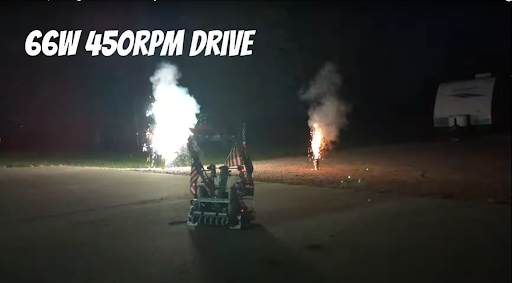
\includegraphics[width=1\linewidth]{images/7686A Independance Day.png}
    \caption{7686A's July 4th Reveal}
    \label{fig:7686A}
\end{figure}



